% NOTES 
% Wie ich den sprinback gemssen habe 

\chapter{Build}

\section{Problem Statement} 
The following design principles is a selection of \cite{siebert_constructionqualitymodel_}'s quality parameters for \ac{ML} models.
In this \ac{DSR} work the artifacts are \ac{ML} models therefore these design principles are used to evaluate them.

\subsubsection*{Design Principle 1: Correctness}
\textit{Does the artifact predict the spring back of a sheet metal with a high accuracy and correctness?}
With progression in manufacturing there is a growing demand for high-quality products, that means that the meta parts needs to be produced with high precision and accuracy. Here the sprin back is an undesired side effect which need to be mimimized. \cite[p. 1]{baig_machinelearningprediction_2021}
Sheet metal forming in manufacturing need a high level of quality and precision. Therefore, the spring back of a sheet metal is an important parameter to consider. \cite[p. 1]{cruz_applicationmachinelearning_2021}
Predicting spring back is important to reduce the number of trial and error cycles in the manufacturing process.
Also predicting spring back is complex because of many variables and parameters and often not all of them are known. 
Therefore, a machine learning model should predict the spring back of a sheet metal with a high accuracy and correctness. When using the \ac{ML} model small errors in the prediction can cause fitting problems in the manufacturing process.

% Using an analytical model to compare the artifact. (miranda 2018 paper)

\subsubsection*{Design Principle 2: Appropriateness}
\textit{Is the artifact appropriate for the given problem?}
While selecting a model it is important that it fits the problem/task and can deal with the given data. \cite[p. 16]{siebert_constructionqualitymodel_}


\subsubsection*{Design Principle 3: Relevance}
\textit{Does the artifact achieve a good bias-variance trade-off?}

In addition to measure the correctness it is important to understand "why" the learner has this performance. 
This is important to understand the limitations of the model and to improve it. 
Therefore, it is important to understand the bias-variance trade-off. \cite[p. 50]{zhou_machinelearning_2021}
Bias measures the differences between the learnesrs expected prediction and the ground-truth label. This results in the fitting ability of the learner. 
Variances measures the change of learning performance of the learner because of changes in the training set. This results in the impact of data disturbance on the results. \cite[p. 51]{zhou_machinelearning_2021}

\subsubsection*{Design Principle 4: Robustness}
\textit{How well does the artifact handle outliers, noise and missing data?}

"Noise is common in any real-world data set and may adversely affect classifiers built under the effect of
such type of disturbance. Some of these classifiers are widely recognized for their good performance
when dealing with imperfect data. However, the noise robustness of the classifiers is an important issue
in noisy environments and it must be carefully studied. Both performance and robustness are two
independent concepts that are usually considered separately, but the conclusions reached with one of
these metrics do not necessarily imply the same conclusions with the other. Therefore, involving both
concepts seems to be crucial in order determine the expected behavior of the classifiers against noise.
Existing measures fail to properly integrate these two concepts, and they are also not well suited to
compare different techniques over the same data. This paper proposes a new measure to establish the
expected behavior of a classifier with noisy data trying to minimize the problems of considering
performance and robustness individually: the Equalized Loss of Accuracy (ELA)."


\subsubsection*{Design Principle 5: Stability}
\textit{Does the artifact generate repeatable results when trained on different datasets?}


\subsubsection*{Design Principle 6: Interpretability}
\textit{Is the artifact easy to understand and explain?}

It should be noticed, that there are many parameters and variables involved in the sheet metal forming process. 
That makes the process design quite complex, particularly in the production of components which require several stages, and thus more than one set of tools. \cite[p. 1]{dib_singleensembleclassifiers_2020}
A model which allows conclusions how the results where generated is better.

\subsection*{Design Principle 7: Resource utilization}
\textit{How many resources does the artifact need to train and predict?}

Conventional processes are often based on empirical trial and error approaches. \cite[p. 1]{dib_singleensembleclassifiers_2020}
A common approach is to experimentally create so named 'technology tables' which contain the bending parameters and the resulting spring back. (Quelle: Hochstrate?)
This process is time and cost intensive and therefore often not suitable for the production of high-volume and low-cost components.
Therefore, one of the benefits of using machine learning should be the reduction of the number of trial and error cycles in the manufacturing process. 
Furthermore, training the model should take not too much time and resources.
As mentioned before often FEM-simulation are used to virtually try out metal forming processes. However, fully exploring the design space is computationally expensive and often not possible. \cite[p. 3]{dib_singleensembleclassifiers_2020} 
The number of experiments can be reduced using a meta-model like \ac{ANN}. \cite[p. 3]{dib_singleensembleclassifiers_2020}
A approach fully based on \ac{ML} should perfor



\section{Dataset generation}
For the dataset generation, bending experiments were performed on metal sheets with different thicknesses.
% material
The material used is cold rolled steel sheets of the norm DIN EN 10130. The thicknesses used were 0.5mm, 1mmm and 2mm.
The material was used because it is commonly used in bending processes and its high availability. In previous tests, it was observed, that the spring back are well observable with this material.
Using this material, 200 single bending pieces of the dimension 20×100 mm have been cut.
Each piece was bend one time using a \textit{Zwick} three-point-bending machine.

Python script where developed to covert the output data format from the machine to CSV files.
The following describes the experimental setup used for the experiments performed.

\subsection{Preliminary Tests}
A number of preliminary tests were conducted to determine the influence of the punch penetration on the spring back.

\subsubsection{Multiple Cycles}
One approach was to test if multiple spring back can be measure using only one sheet.
Therefore, the machine was programmed to perform multiple cycles in one attempt and bend the metal sheet multiple times. The benefit of this approach would have been a faster generation of the dataset because spring backs could be measured in on attempt, also less material would have been used.

Figure~\ref{springback_multiple} shows one of these attempts. The metal sheet was bent 4 times using $y_p$ values from 5 to 8. The results show, that 4 different spring backs can be measured, but the spring back does not vary like expected. It was observed as well, that the spring backs are different in every attempt, this is shown in Figure~\ref{springback_multiple_inconsistent_results}.
Bending 4 different metal sheets each only one time returned very different results.
A possible explanation could be the cold deformation of the steel, which is not reversible. Because this approach did not work, the machine was programmed to perform one cycle at a time.

\captionsetup{width=0.45\textwidth}

\begin{figure}[H]
    \centering
    \begin{minipage}[b]{0.5\textwidth}
        \centering
        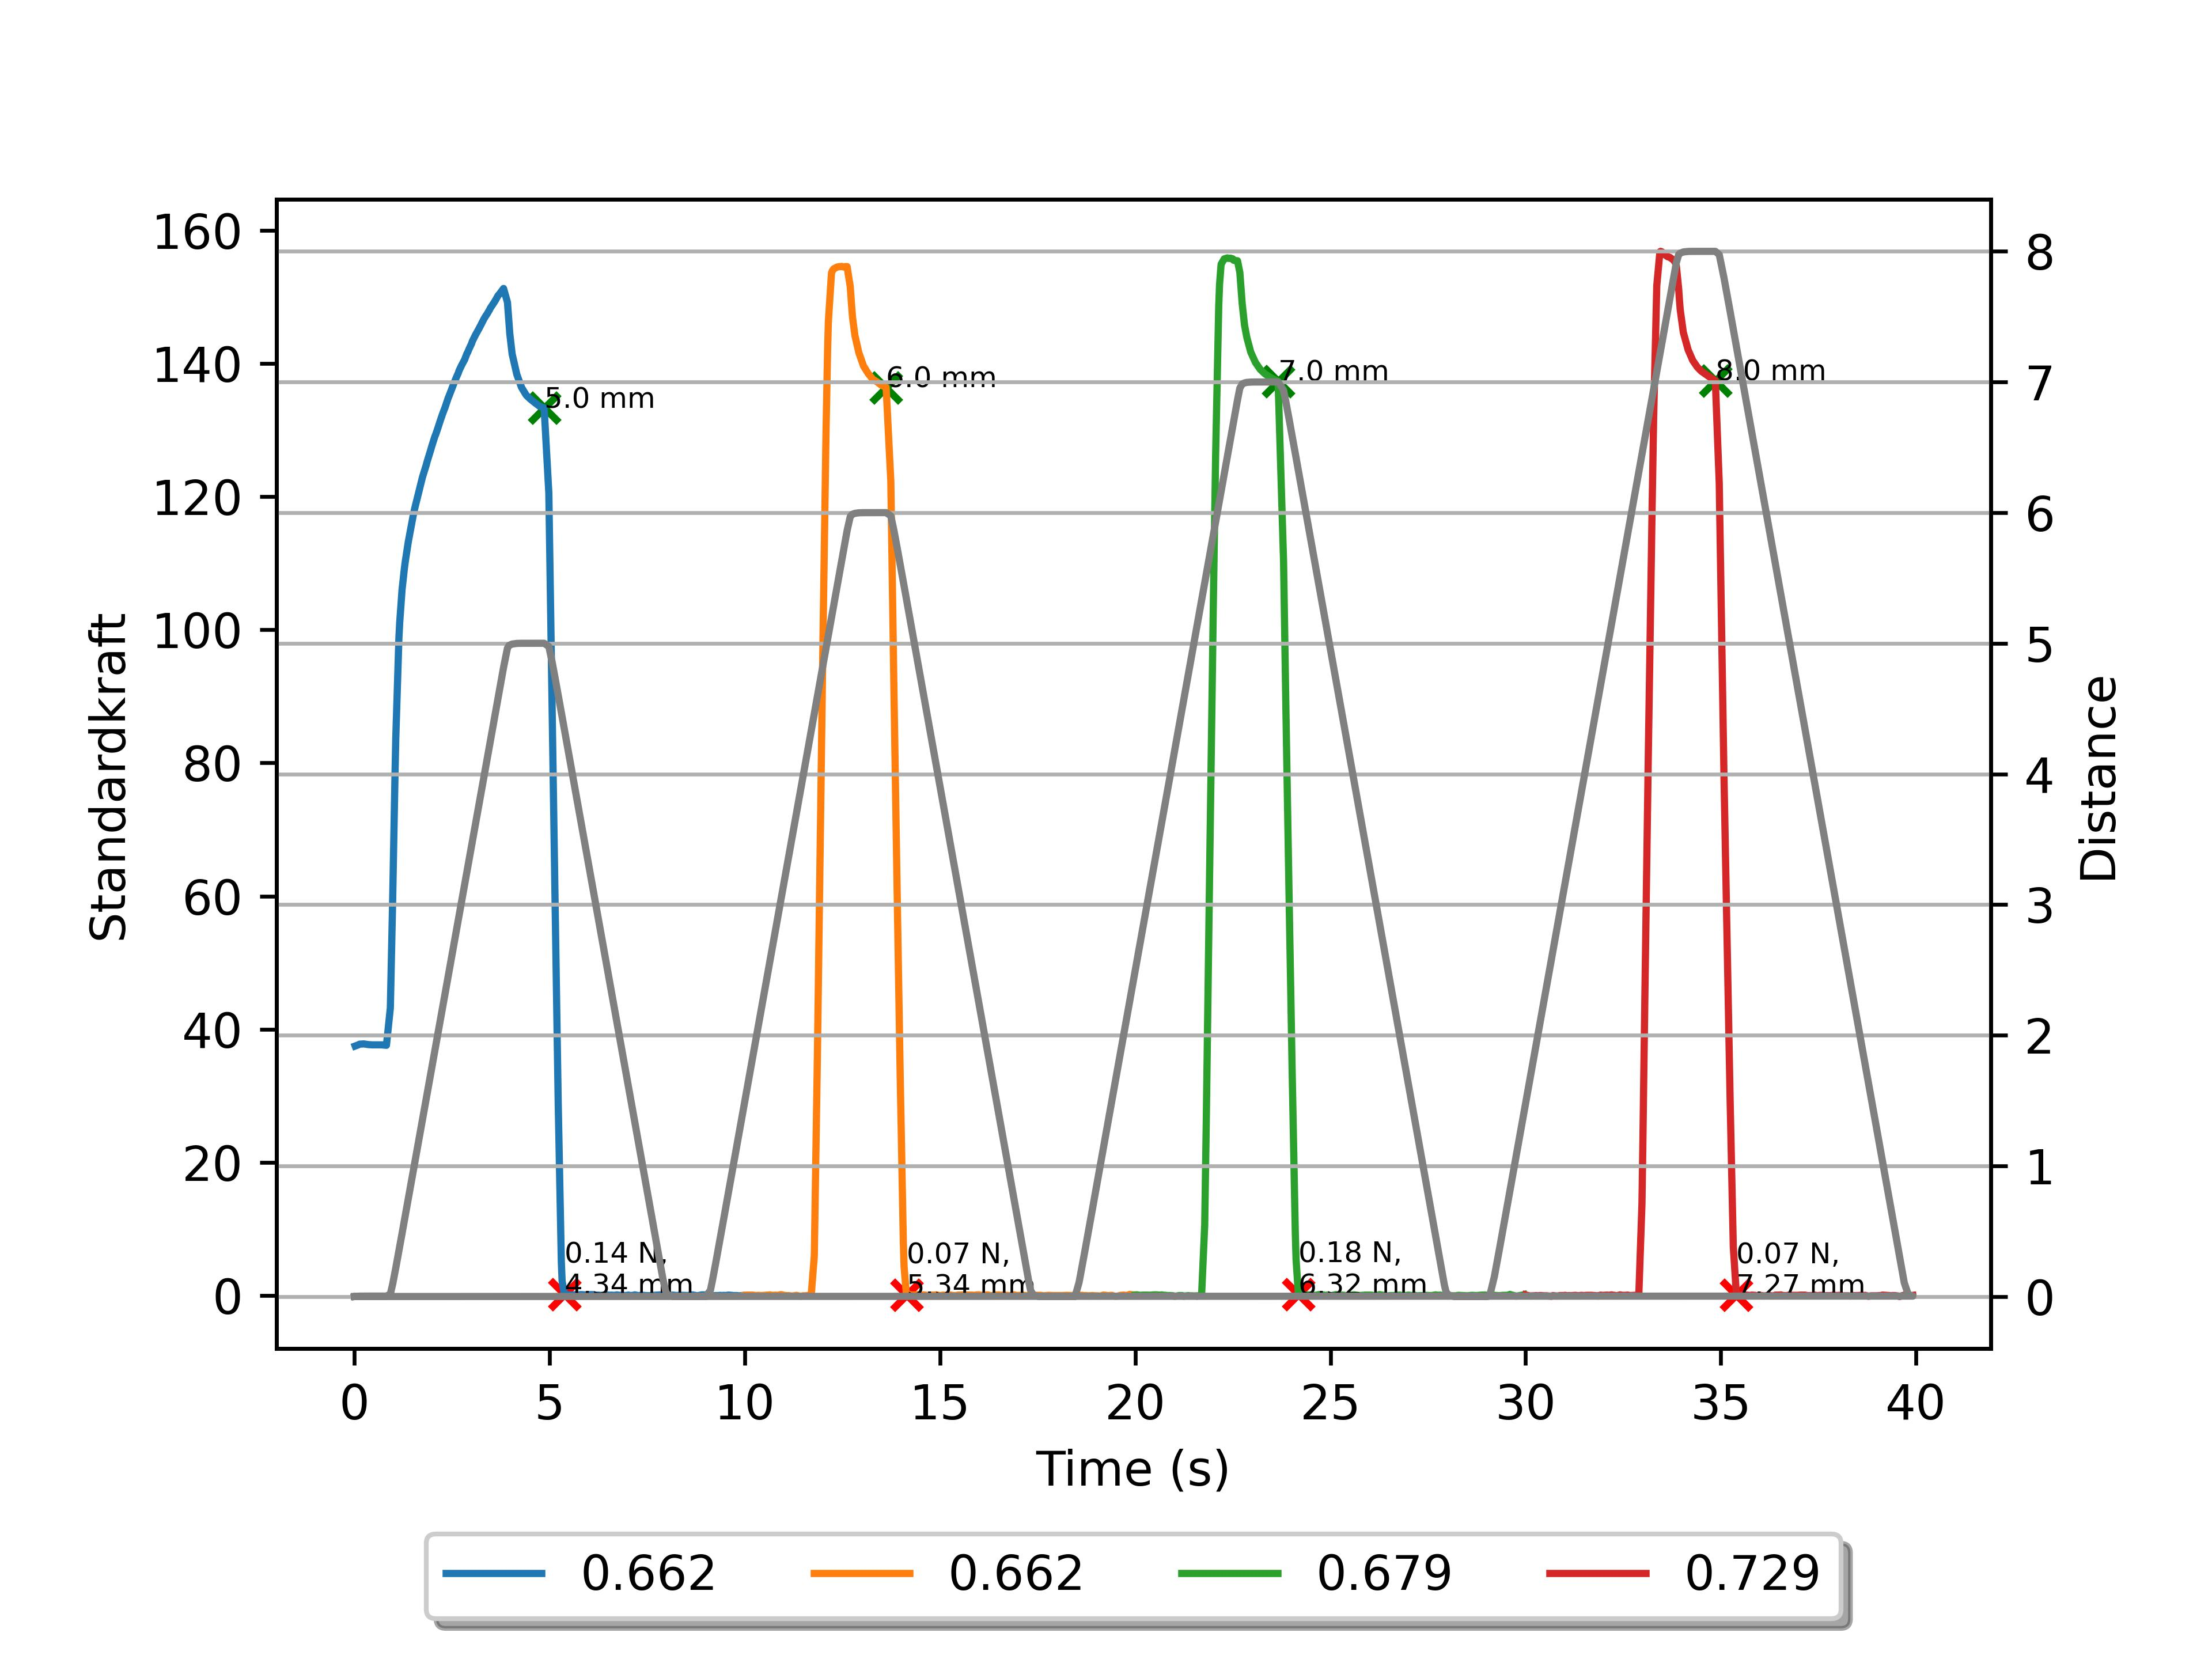
\includegraphics[width=0.9\textwidth]{springback_multiple.jpg} % first figure itself
        \caption{Experiment: Bending one metal sheet multiple times with different $y_p$ values.}
        \label{springback_multiple}
    \end{minipage}\hfill
    \begin{minipage}[b]{0.5\textwidth}
        \centering
        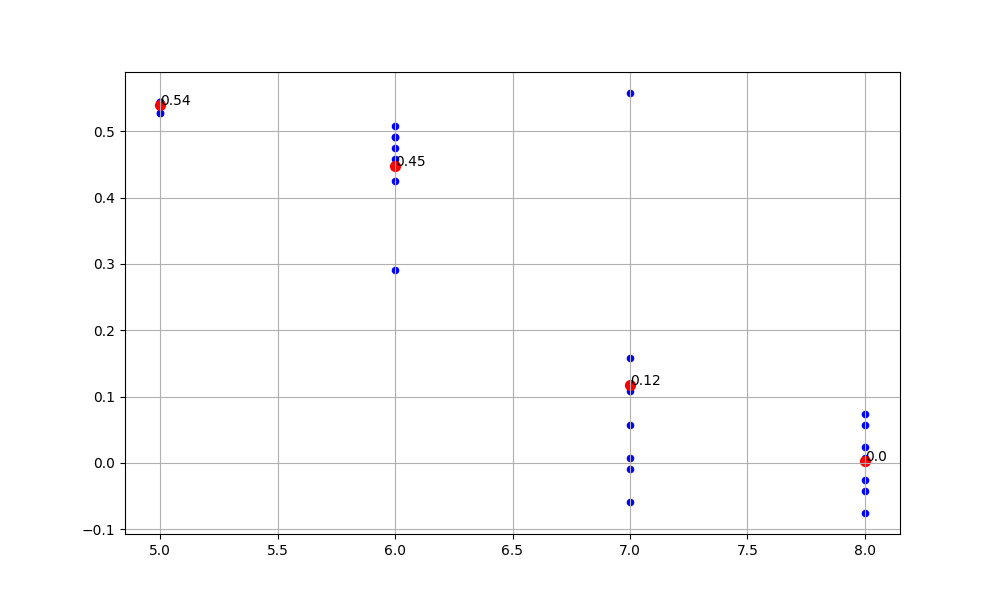
\includegraphics[width=1.1\textwidth]{springback_multiple_inconsistent_results.png} % second figure itself
        \caption{Inconsisten results bending one metal sheet mutliple times. The spread of the results is very large.}
        \label{springback_multiple_inconsistent_results}
    \end{minipage}
    \label{fig:springback_multiple_overview}
\end{figure}

\subsubsection{Brake Bending Machine}
Before using the three point bending machine, a brake bending machine was used to test the influence of the bending on the spring back. The brake bending machine is a machine used to bend metal sheets. It is a very common machine in the industry and is used to bend metal sheets to a specific radius. The brake bending machine used is a \textit{Bendmaster 1000} from \textit{Bendmaster}.

After a series of bends it was observed, that the spring back values where much higher than expected. The explanation for that behavior was, that altering the position the bending beam of that specific machine was not enough to get the desired angle. Thus, the machine excluded for the generation of the data and the three point bending machine was used instead.

Despite the inaccurate data, it was later observed, that the distribution of the spring backs was very similar to the later experiments with the three point bending machine.


\subsection{Experimental setup}
The setup consists of a three-point-bending machine with a punch and a die with no bottom. The machine used is the \textit{Zwick MX 25A} material testing machine.
The machine is equipped with a load cell and a displacement sensor. The load cell is used to measure the force applied to the sheet and the displacement sensor is used to measure the displacement of the punch.
The machine is controlled by a computer and a software called \textit{ZwickRoell TestXpert}. The software is used to control the machine and to save the output data.

The experimental setup and the process parameters are shown in Figure~\ref{fig:setup} where $V$ is the die opening, $y_p$ is the punch penetration which is the distance the punch is moved into the sheet.
The paramter $t$ is the sheet thickness,  $\alpha$ is the sheet corresponding bending angle. Parameter $r_p$ is the punch radius which is the radius of the tip of the punch and $r_m$ is the die radius.


\begin{figure}[H]
    \centering
    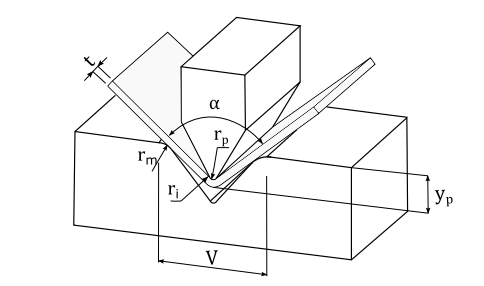
\includegraphics[width=0.6\textwidth]{setup}
    \caption{Process parameters: Sheet bending angle ($\alpha$), sheet thickness ($t$), punch penetration ($y_p$), die opening ($V$), punch radius ($r_p$), die radius ($r_m$), inside bending radius ($r_i$).}
    \label{fig:setup}
\end{figure}

In order to get consistent results, a number of constant and variable parameters were chosen.
The parameters include the punch-and-die tooling made of steel where die punch had a radius ($r_p$) of 5 mm and and die radius ($r_m$) of 10 mm. The die opening $V$ was varied between 10 and 50 mm and the punch penetration $y_p$ was varied between 0 and 20 mm.
The machine was configured to move the punch with a constant speed of 100 mm/min until it measured a resistance of 1 N. That meant, that the punch reached the metal plate and the actual bending process can start. After a hold time of 1 second the punch was moved with a slower speed of 8 mm/min until the specified punch penetration was reached.
The length and width of the metal sheet was 100 mm and 20 mm respectively. The sheet thickness was varied between 0.5 and 3 mm.
The constant parameters are shown in Table~\ref{tab:constant_parameters} and the varying parameters are shown in Table~\ref{tab:verying_parameters}.

\begin{table}[H]
    \centering
    \begin{tabular}{|l|l|l|}
        \hline
        \textbf{Parameter} & \textbf{Value}                      & \textbf{Unit} \\ \hline
        Punch penetration  & 2.5, 5, 7.5, 10, 12.5, 15, 17.5, 20 & mm            \\
        Die opening        & 10, 20, 30, 40, 50                  & mm            \\
        Thickness          & 0,5, 1, 1.5, 2, 2.5, 3              & mm            \\
        \hline
    \end{tabular}
    \caption{Experimental setup varying parameters}
    \label{tab:verying_parameters}
\end{table}

\begin{table}[H]
    \centering
    \begin{tabular}{|l|l|l|}
        \hline
        \textbf{Parameter}            & \textbf{Value} & \textbf{Unit} \\ \hline
        Punch radius                  & 5              & mm            \\
        Die radius                    & 5              & mm            \\
        Sheet thickness               & 0.5, 1, 2      & mm            \\
        Sheet width                   & 20             & mm            \\
        Sheet length                  & 100            & mm            \\
        Punch speed                   & 100            & mm/min        \\
        Punch speed after penetration & 8              & mm/min        \\
        Punch force                   & 1              & N             \\
        \hline
    \end{tabular}
    \caption{Experimental setup constant parameters}
    \label{tab:constant_parameters}
\end{table}


\subsection{Measuring The Spring Back}
The output data contained different data points, which were used to calculate the spring back.
Important parameters for the calculation are the force, punch penetration and testing time.
As shown in Figure~\ref{fig:springback_measured} at the $yp$ maximum the punch penetration and the force are maximized as well. The punch stays at that position for 1 second and then moves back with a slower speed. This hold time a limitation of the machine and can not be changed.
After the punch is moved back, the force is reduced and the punch penetration is reduced as well, until the punch is at the initial position. For a short time after the lift, the load  cell still measures a force. That is because the metal sheet springs back and the punch is still in contact with the sheet. This was measured using a python script, the green and the yellow point represent the resulting spring back distance.

\begin{figure}[H]
    \centering
    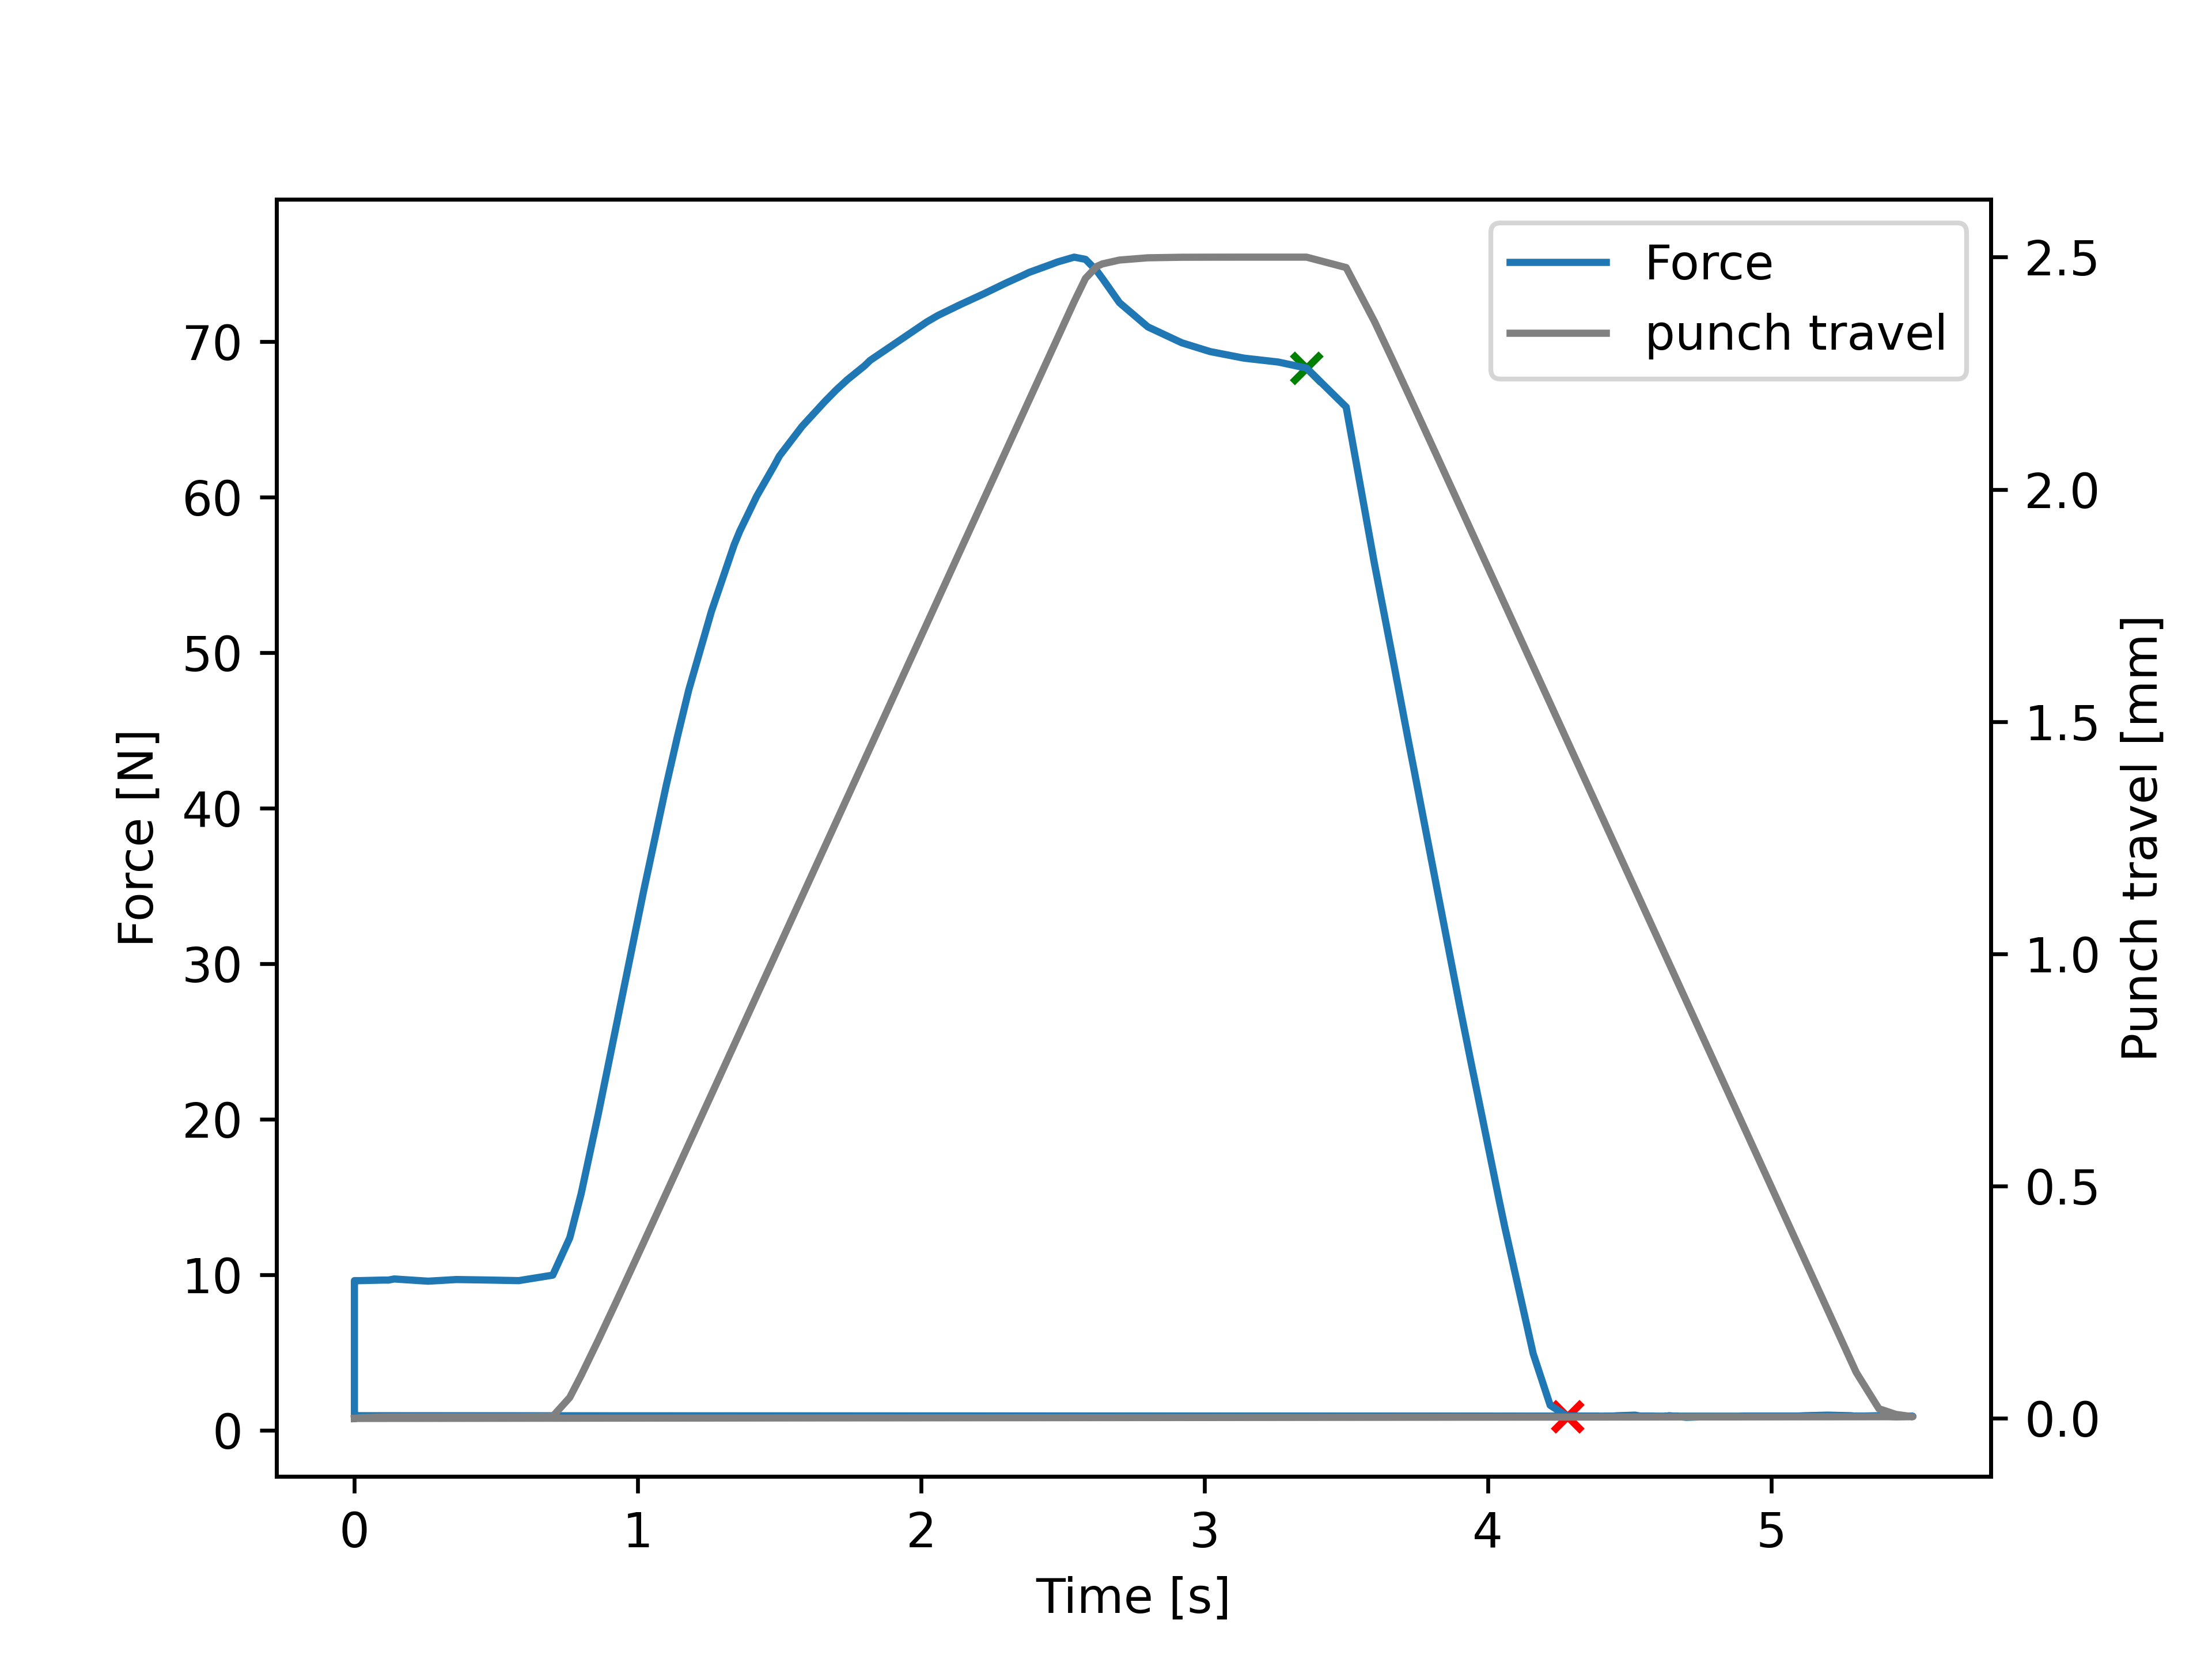
\includegraphics[width=0.6\textwidth]{springback_measured}
    \caption{A steel metal sheet was bent with a punch penetration of 5 mm the spring back is 0.37 mm. The blue line shows the force and the blue line shows the punch penetration.}
    \label{fig:springback_measured}
\end{figure}

% \paragraph{Bend deduction:}
% Measuring the bend deduction is more complex. After a metal sheet is bent, it is hard to measure the flat pattern length because the material is malformed at the bent. 
% As a result, the neutral axis is not in the center of the sheet and hard to measure, but it can be calculated using different approaches. %quelle und ausführlicher und grunlagen teil  
% There are multiple ways to measure the bend deduction described earlier. 
% % K-Faktor Muss noch in theorie teil 
% In this setup, the method described in the DIN6395 was used. This method uses a k-factor which is an approximated value and therefore and therefore it can be inaccurate. (Equation~\ref{eq:kfactor}). % cite DIN norm 

% \begin{equation}\label{eq:kfactor}
%     k=0.65+\frac{1}{2}\log{\frac{r}{s}}
% \end{equation}

% \begin{figure}[ht!] % supposedly places it here ...
% 	\centering
% 	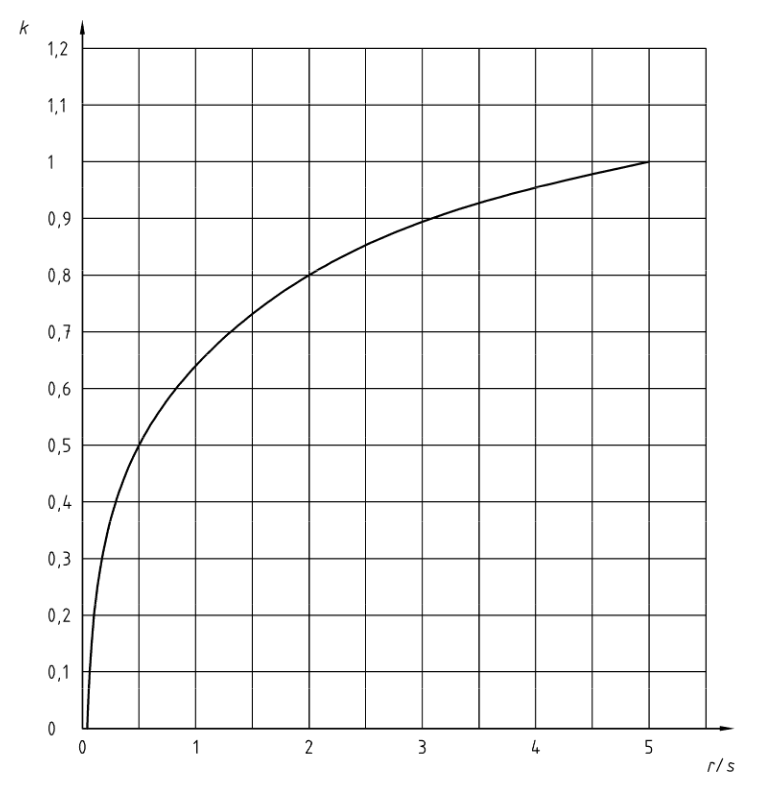
\includegraphics[width=0.5\linewidth]{k-factor}
% 	\caption[Graphical representation of the correction factor]{Graphical representation of the correction factor.}
% 	\label{fig:test1}
% \end{figure}

% The DIN 6935 used the formula for the stretched length, $length=a+b+v$ where \textit{a} and \textit{b} are the side lengths of the sheet and \textit{v} is a correction value for the deduction. \cite{din6935}
% The stretched length is measured different depending on the bending angle.

% \paragraph{Opening angle $\beta 0^\circ$ to $90^\circ$} 
% For opening angles between $0^\circ$and $90^\circ$ the side lengths \textit{a} and \textit{b} are dimensioned from the tangent of the bend to the edge. 
% To calculate the compensation value \textit{v} (Equation~\ref{eq:v1}) is used
% \cite{din6935}.

% \begin{equation}\label{eq:v1}
%         v=\pi*(\frac{180^\circ-}{180^\circ})*(r+\frac{s}{2}*k)-2(r+s)
% \end{equation}

% \begin{figure}[H]
% 	\centering
% 	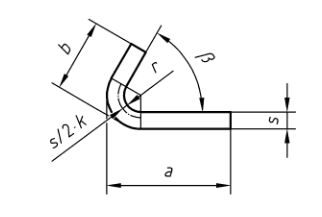
\includegraphics[width=0.5\linewidth]{bending-angle-90}
% 	\caption[Opening angles $\beta 0^\circ$ to $90^\circ$]{Opening angles $\beta 0^\circ$ to $90^\circ$ \cite{din6935}}
% 	\label{fig:v1-image}
% \end{figure}

% \paragraph{Bending angle $\beta90^\circ$ to $165^\circ$} (Equation~\ref{eq:v1})
% For opening angles between $90^\circ$ and $165^\circ$ the side lengths \textit{a} and \textit{b} are dimensioned from the apex to the edge. 
% To calculate the compensation value \textit{v} (Equation~\ref{eq:v1}) is used. 
% \cite{din6935}

% \begin{equation}\label{eq:v2}
%     v=\pi*(\frac{180^\circ-}{180^\circ})*(r+\frac{s}{2}*k)-2(r+s)+\tan{\frac{180^\circ-\beta}{2}}
% \end{equation}

% \begin{figure}[!ht]
% 	\centering
% 	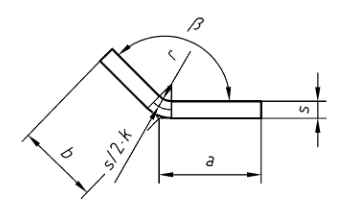
\includegraphics[width=0.5\linewidth]{bending-angle-165}
% 	\caption[Opening angles $\beta90^\circ$ to $165^\circ$]{Opening angles $\beta90^\circ$ to $165^\circ$ \cite{din6935}}
% 	\label{fig:v2-image}
% \end{figure}

% For opening angles between $165^\circ$ and $180^\circ$ the compensation value \textit{v} is 0. The values for v would be negligibly small. \cite{din6935} The side lengths \textit{a} and \textit{b} where measured using the software \textit{ImageJ}. 

% Edge cracking is not measured for now because the steel used has no high-strength and with machine in usage it was not possible to create edge cracking.

% \begin{figure}[!ht]
% 	\centering
% 	\includegraphics[width=0.5\linewidth]{example-image}
% 	\caption[Screenshot ImageJ]{Screenshot ImageJ}
% 	\label{fig:imagej-screenshot}
% \end{figure}


\subsection{Computational Setup}
For training the machine learning models a ThinkPad X1 Carbon 2019 with an Intel Core i7-10610U CPU @ 1.80GHz and 16 GB RAM was used. The operating system used is Ubuntu 20.04.2 LTS. The code for the model is written in Python 3.8.5 using the IDE PyCharm The libraries used are mentioned in Table

\captionsetup{width=1\textwidth}

\begin{table}[H]
    \centering
    \begin{tabular}{|ll|}
        \hline
        \textbf{Library} & \textbf{Version} \\
        \hline
        numpy        & 1.23.2  \\
        pandas       & 1.5.1   \\
        matplotlib   & 3.6.2  \\ \hline 
    \end{tabular}
    \label{table:libraries}
    \caption{Libraries used for the machine learning models.}
\end{table}

\subsection{Data Preprocessing}
% "Although the dataset collected from the experimental setup includes seven features (parameters), the 
% first three parameters; load tonnage, load holding time, and gap between the punch and the die, are 
% combined to form a single feature, "Machine". It is because different combinations of these factors may 
% be combined to form a single machine setting parameters. The other parameters are; blank material, 
% thickness, width and initial bend angle. Hence, there are five features of the dataset, which levels are 
% shown in Table 4. Two of which, namely machine and material, are treated as categorical features, so 
% using scikit-learn's OrdinalEncoder these features were encoded into an integer array. While the 
% remaining three features were treated as continuous features, for standardizing these features scikit-
% learn's StandardScaler was used. It transformed the data so that for each feature, its distribution 
% will have a mean value of 0 and a standard deviation of 1. The formula used for this is as follows Eq 
% (1)." 
% \cite[p. 7]{baig_machinelearningprediction_2021}

\section{Model Selection}

\begin{itemize}
    \item Multi-layer Perceptron (MLP)
    \item Decision Tree (DT)
    \item Random forest (RF)
    \item Naive Bayes (NB)
    \item Support vector machine (SVM)
    \item K-Nearest neighbors (KNN) 
    \item Logistic Regression (LR)
\end{itemize}

\section{Model Training}








